\chapter{Introduction}
\label{ch:intro}

\section{Space and navigation as abstract concepts of everyday life}
\label{sec:navig_in_life}

For about a decade I was curious whether reading books from an electronic device is anyhow affecting comprehension or learning, an ability to remember facts, events or their sequence - compared to their paper versions. The modern electronic way of reading exposes many advantages: you can store 1000 books in the same small device, you can quickly search any text by a word, there is an ability to make notes and highlight valuable fragments and, of course, to share all that content between physical devices. These advantages were by far overtaking and convincing towards using electronic versions for reading until I found the research on reading comprehension by \cite{Mangen2013}. They demonstrate that text comprehension was lower for the group of electronic readers, compared to the paper-based readers, and that it is mostly related with the reduced ability to reproduce the sequence of described events for narratives or locating information in texts in general (\cite{GiuliaCataldo2000}). Interestingly, the major hypothesis for the decrease of performance is the reduced spatial representation of the electronic book compared to the printed content (\cite{Mangen2013}). They argue that access to paper texts comes in a coherent combination of visual and tactile cues, allowing a reader to build spatial extension and physical dimension of the text. This is supported by earlier empirical and theoretical studies showing that a good mental spatial representation of the text layout supports reading comprehension (\cite{Kintsch1998}; \cite{PIOLAT1997565}). So building a good spatial representation of the content is important for comprehension and learning.

How else do the abstract concepts of space and navigation have an impact on our life? Let’s jump to the world of classical music and imagine a musical piece. A set of notes (tones) can be taken as a particular music space (e.g. the standard 88 keys on the piano keyboard). A melody, from note to note, accompanied by chords and passages, builds a trajectory in this imaginary music space. This music space has a physical projection called sheet notes, usually printed on paper. While reading sheet notes of a particular piece, we go through the special signs and symbols - “forte” or “piano”, “fermata”, “rest”, “coda” and others, which act as visual cues and landmarks in the current music trajectory. So what is essential to be able to play a music piece? It is inevitable to build a mental representation of the music space in the brain, as well as to be able to navigate in that music space, by learning and executing existing or building new “music” trajectories and linking them to the physical arm and finger actions - depending whether you prefer piano, violin or a guitar (see also “Mental play” in \cite{ChuanChang2016}).

A game of chess is another example of an abstract space, a bit closer to the classical physical “real-world” space representation. The chessboard has its strictly defined boundaries and spatial positions. Direction and type of movements in the chessboard space are predetermined for different actors and also limited depending on the position of other figures. The victory in a game is critically dependent on the ability to build a reliable representation of that chessboard space in the brain, as well as to build a magnitude of possible trajectories that, one after the other, could be implemented by figures of both colors.

Abstract concepts of space and navigation are applicable to many physical modalities. Besides the traditional spatial navigation from a bedroom to a kitchen, from home to work or from Munich to Moscow, we constantly need to solve spatial problems in relative spaces - like to define on which shelf relative to the freezer should I put back a coffee cup, or to imagine somewhere away to the far left in the egocentric space when locating a source of a pleasant sound (see also Buzsáki, 2019, “Space in the world versus space in the brain”). What do all these physical or abstract “spatial” tasks have in common? At the high cognitive level, the implementation of all these types of spatial navigation mostly located in the medial temporal lobe, specifically in the hippocampal-entorhinal system. Having location- and spatial cue-selective neurons (\cite{OKeefe1978}, \cite{Moser2015}), hippocampus and parahippocampal cortex together are able to form representations of not only physical spatial dimensions, but act as a general machinery for building arbitrary representations of physical and abstract spaces (\cite{Aronov2017}). These  mental cognitive maps - dynamic ensembles of cells selective for combinations of physical or abstract spatial features representing unique locations or experiences - are necessary to build and implement navigation in these spaces, potentially via sequential activation of these neural ensembles in a form of mental trajectories (\cite{Hopfield2010}; \cite{Buzsaki2018}).

Up to the moment, the exact mechanisms how these neuronal dynamics are implemented at both  population or single neuron level is still not fully understood. In this work, I’m trying to contribute to the research on navigation in physical space as a special subclass of cognition tasks implemented by the hippocampal-entorhinal system.


\section{Spatial representation in the hippocampal-entorhinal circuit}
\label{sec:spatial_repr}

Spatial navigation in mammals is implemented as a cooperative dynamic neural network, distributed across multiple brain regions. This network encodes not only an allocentric position in space, but also movement direction, as well as the past and future trajectories. The great evidence for it are the discoveries of place cells, grid cells, head direction cells and other types of spatial feature selective cells, located mostly within the hippocampal, parahippocampal and entorhinal brain areas (see review in \cite{Moser2015}). Place cells were defined mostly as neurons selective to a particular location in an environment. Grid cells, one synapse away from the place cells, are also place selective neurons but that are active not at single locations, but at a regularly-spaced intervals, bringing a periodic structure to the physical space inside the cognitive brain map. Place cells are modulated by a variety of inputs, including external visual landmarks, olfactory or tactile cues, translational and rotational signals and integrated proprioceptive signals, which allow them to maintain activity of their place of preference when the sensory signals are absent, like in the absence of light. While place cell activity can unpredictably change from one environment to the next (\cite{Colgin2008}), in contrast, grid cells keep their firing independent of the individual details of a particular environment (\cite{Fyhn2007}), providing a putative metric of space. Additionally, orientation in the environment can be taken from the head-direction system, implemented by the neurons located in different brain areas but importantly in the post-subiculum, and being active when the animal's head is pointed to a certain direction (\cite{Taube2007}). More specific cell types, like boundary-vector cells, or cells responding to a combination of environmental features (\cite{Deshmukh2013}; \cite{Hooydal2019}) extend the navigation system in fine-tuning actual position estimation, in correcting accumulated positional errors and perfecting future spatial planning. Below, there is a short review of each of the particular cell types and its possible involvement in the brain navigational system. As the exact internal organization of the navigation system is not fully defined yet, at the end of this chapter I discuss open questions and focus on the yet unknown parts of it that I try to address and to make a contribution to in this study.

\subsection{Place cells}

Hippocampal cells responsive to a current location of an animal were first found by O’Keefe and Dostrovsky in 1971. After the discovery, these cells acquired a name of “place cells” (Figure 1a). Although there are many ways of the functional organization in the cortex - like the topographic organization in the visual area V1 (\cite{Schuett2002}), place cells in the CA1 area appeared to not form any simple organizational pattern, such that the neighboring cells may represent different locations and features of the environment. Later it was discovered that the size of the environment, selective for a particular place cell, varies from the cell location within the hippocampus, from dorsal (smaller, precise fields) to ventral (lager fields, \cite{Jung1994}). The emerging interest to the hippocampal research after the place cell discovery led to the discovery of the hippocampal neurons responding to non-spatial features, like odors (\cite{Wood1999}; \cite{Igarashi2014}), border and general tactile information (\cite{Young1994}; \cite{Okeefe1996}), distance or timing (\cite{Hampson1993}; \cite{Kautzky2016}). However, although much of the hippocampal findings relate to the representation of space, it does not limit the role of the hippocampus in declarative memory in general - place representation is just a key element in many episodic or even semantic memories (\cite{Buzsaki2013}).

Importantly, the recordings of hippocampal neurons in novel environments reveal that the majority of place cells appear to have immediate firing fields (\cite{Frank7681}). Although several studies of hippocampal ensembles demonstrate, that often the formation of stable fields takes up to several minutes (\cite{Wilson1993a}), this presence of immediate fields suggests that certain components of the network are pre-wired in the circuit, and that the basic elements (neurons, synaptic connections) of the cognitive map are largely predetermined.
In short summary - place cells provide dynamic and continuous information about the animal’s position in space, and together, on the population level, these cells are able to form a cognitive map - an abstraction in the brain that represents allocentric space.

\begin{figure}
\captionsetup{format=plain}
\makebox[\textwidth]{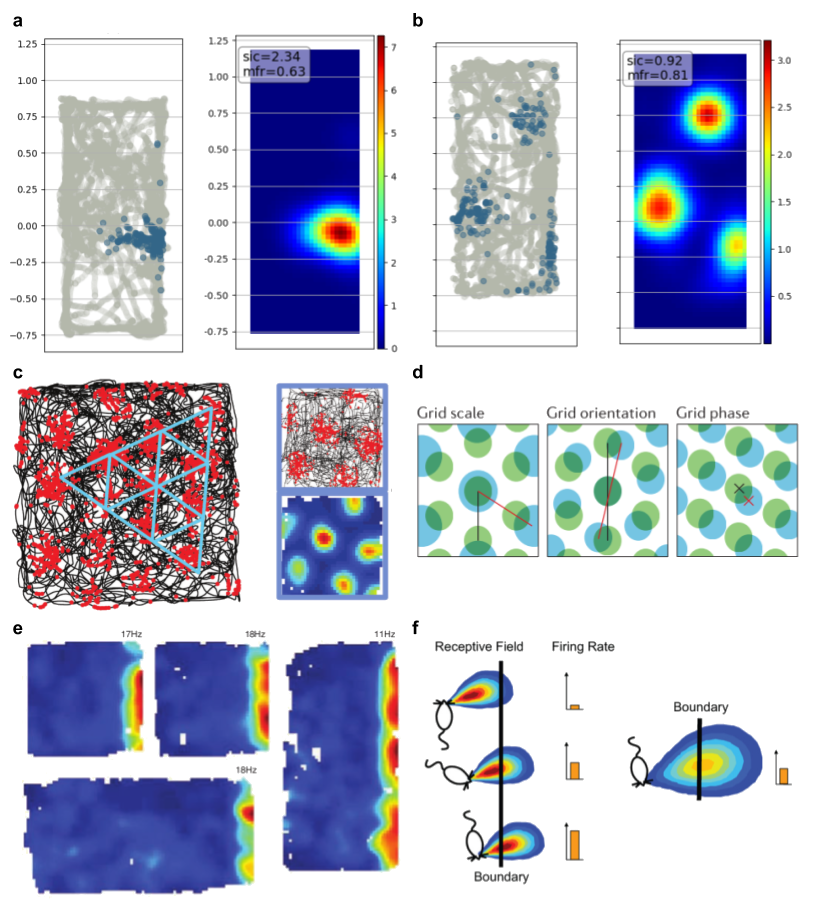
\includegraphics[width=150mm]{figures/F1_place_cells.png}}
\caption[Place and grid cells]{
Place, grid and border cells. \textbf{(a)} Firing rate map of an example hippocampal neuron that is active at a certain location in the rectangular environment - a “place” field. \textbf{(b)} another example neuron that has multiple place fields of different size (examples from the data used in the current study). \textbf{(c)} Firing rate map of an example mEC neuron that is active at certain locations of the environment, that form a hexagonal grid pattern (left). Place preference autocorrelograms reveal hexagonal structure (Adapted with permission from \cite{Moser2015}) \textbf{(d)} Examples of pairs of grid cells having different scale, orientation and phase (adapted with permission from \cite{Moser2014}). \textbf{(e)} Firing rate maps of an example neuron that is active near the right border of the environment, invariant of the environment type (adapted with permission from \cite{Solstad2008}) \textbf{(f)} schematic of the receptive field of an example neuron that is selective for a particular direction and distance to the environmental boundary (\cite{Lever2009}).
}
\label{fig:F1_place_cells}
\end{figure}


\subsection{Grid cells}

In addition to the discovery of the place cells, a few decades after, another important type of the place-selective cells were found in the brain’s entorhinal cortices. Particularly, in the layer II of the Medial Entorhinal Cortex (mEC) neurons, forming discrete regularly spaced firing fields were identified (\cite{Hafting2005}). Surprisingly, the firing fields of those neurons were organized in a grid of tessellating triangles evenly covering the corresponding space (Figure 1c). A simple autocorrelogram analysis revealed the rigid hexagonal structure (Figure 1c right). Key features of the newly discovered cells were, first - their different spacing between individual fields and phase shift relative to each other, with the increasing scale from dorsal to ventral mEC, and second - their anchoring to the boundaries, persistence between environments and independence on visual or olfactory landmarks. These facts suggest this type of cells is primarily based on self-motion and plays a main role in path integration, mixing idiothetic vestibular and proprioceptive signals.
Anatomically, mEC has a direct input to the Hippocampus. This led to the assumption that grid cells, sharing common peak and different spacing, might be a good basis to form place cells, taking grid cell inputs as a linear combination (\cite{OKeefe2005}). However, experimental evidence, based on studies on developing animals, shows that mechanisms are more sophisticated, as there is a delayed maturation of the grid fields relative to place cells. An alternative assumption, that place cells can be formed as a combination of the grid and other cell-type inputs - like border cells (see below), which are ready at the early stages of the development, looked to be more consistent. As suggested (\cite{Savelli2008}), specific place cells may arise as neurons integrating inputs from grid cells that provide proprioceptive-based distance information, and border cells that provide position relative to external boundaries. This putative idiothetic place cells will be named “boundary-driven” or “boundary-vector” cells later in the text.


\subsection{Head direction system}

One of the key components for successful navigation is maintenance of the proper allocentric orientation. Even before grid cells, neurons, which firing rates depend on the animal’s head orientation were found - originally in postsubiculum (\cite{Taube2007}), and later in other nearby areas (mEC, AdN etc.). Besides their primary feature of keeping the absolute directional preference, the “head-direction” cells were shown to maintain their relative directional preferences between each other; however, each cell by itself has no particular preference in absolute world coordinates - its directional preference can change between different environments. Importantly, in absence of light, head direction cells are able to integrate angular velocity of the head and maintain original directional preference, although for the cost of accumulation of directional error.

The presence of head direction cells is a necessary part to perform successful path integration, especially when light or external allocentric sensory cues are not present. The interaction of grid cells, providing distance estimation and a metric for space based on idiothetic inputs, and head direction cells supplying absolute orientation define the basis for position estimation based on path integration, which  is discussed more in one of the next sections of this chapter.


\subsection{Border and BVC cells}

While grid cells and head direction cells provide distance and orientation estimation, respectively, actual position should be estimated in relation to a certain point in space - usually relative to a physical boundary. Further research of the cell functions in the mEC lead to a discovery of the neurons representing geometric boundaries (\cite{Solstad2008}), and cells active at a particular distance to a certain boundary. These “border” and “boundary” cells are active when an animal is located near a certain physical boundary; their firing is independent of affine transformations (Figure 1e). A border cell, or more generally, a putative boundary vector cell (\cite{Barry2006}, \cite{Lever2009}), is another type of the neuronal encoding found in the mEC, that is involved in spatial representation. In a series of recordings these cells demonstrated preference to fire at a certain distance and direction to a particular object (Figure 1f) or, as a special case, to a certain boundary.

Border and boundary-vector cells (BVCs) may play an important role in updating positional signals of grid cells, as the latter tend to drift in open spaces. If the animal hits the boundary, any accumulated error in the grid cell positioning can be “reset” and appropriately corrected (\cite{Hardcastle2015}). Taken together, by defining the perimeter and stable physical objects relative to this perimeter inside, border and object-vector cells may represent an independent reference frame that can be used later by place cells to form correct space representations in the hippocampus.


\subsection{Landmark and object vector cells}

Besides environmental boundaries, stable visual landmarks can be used for building navigational strategies. In the visual sensory domain, cells, selective for certain spatial landmarks were discovered in the lEC (mEC) (\cite{Deshmukh2011}; \cite{Kinkhabwala2020}), and later in the CA1 and CA3 (\cite{Deshmukh2013}). These different selectivity types are ranging from an increase of neuron’s activity when passing a certain visual cue on the linear tracks (\cite{Kinkhabwala2020}), up to forming a stable firing field relative to a landmark at a certain distance and orientation. This discovery was further developed to a concept of general object vector cells found in the mEC, pointing to an idea that vector coding is a dominant form of position coding the entorhinal system (\cite{Hooydal2019}).


\subsection{Anatomy of the hippocampal-entorhinal system}

To establish meaningful conclusions about the mechanisms of the spatial navigation system, it’s important to explore the basic anatomical and functional connectivity of the underlying brain regions. Below we provide an essential extraction from the review of the anatomy of the hippocampal formation and the entorhinal cortex regions as the key areas involved in navigation, based on the rodent brain.

First we focus on the sagittal view of the rat’s right hemisphere, a horizontal brain slice in the middle of the hippocampal formation (Figure 2a). The hippocampal formation is presented by the key areas CA1, CA2 and CA3, as well as the DG and Subiculum. Darker areas show a density of pyramidal cell types (stratum pyramidale), where most of the place selective hippocampal neurons are found; lighter areas mostly contain dendrites and interneurons. The Parahippocampal region is represented by lEC, mEC, PrS and PaS areas. These regions contain the aforementioned grid cells and boundary-vector cells, as well as neurons selective to absolute orientations.

Pyramidal cells are excitatory cells that use Glutamate as a neurotransmitter. Different types of interneurons are all GABAergic (inhibitory), having their cell bodies distributed within all layers of the hippocampal formation (stratum radiatum, pyramidale, lacunosum-moleculare, oriens). Importantly, the activity of pyramidal cells are modulated by both external (e.g. mEC neurons) and internal (like CA3 principal cells and local inhibitory interneurons) inputs. One can distinguish principal cells and interneurons from electrophysiology. Principal cells have larger action potentials, have in average lower mean firing rate, and show noticeable bursty behavior.

The main cortical input to the hippocampus is the input from the entorhinal cortex that goes via the perforant pathway. Essentially this input conveys pre-processed information from higher-order sensory and association areas. In particular, most of the neurons of the layer 2 of the EC project to the DG and CA3, at the same time neurons in the layer 3 find their targets in the CA1 and Subiculum. CA1 and Subiculum provide feedback connections to the EC layer 5. There is a complex topography: all entorhinal layers are reciprocally connected (Figure 2b). In addition, there is also a mEC projection to the contralateral hippocampus with the same topography, although of a smaller density.

In essence, in the context of formation of place cells, the presented hippocampal-entorhinal connectivity allows for integration of the different mEC / lEC types of inputs with local CA3 inputs at the level of the CA1 pyramidal cells. This forms an anatomical basis for the assumption of the integration of grid, or boundary-vector cells, coming from the EC, with sensory driven cells - like visual landmark cells for the transient formation of the stable spatial representation in the form of place cells in the CA1 region.

\begin{figure}
\captionsetup{format=plain}
\makebox[\textwidth]{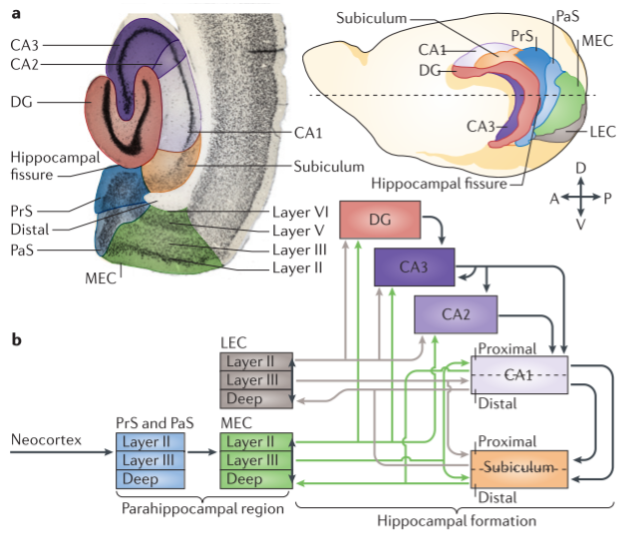
\includegraphics[width=150mm]{figures/F2_HPC_anatomy.png}}
\caption[Hippocampal-entorhinal Anatomy]{
(a) A slice of the right hemisphere of the rat brain (left). The focus is made on hippocampal and entorhinal regions. The same regions are shown located inside the rat brain (right). (b) Schematic of the connections within and between hippocampus and entorhinal cortex (adapted with permission from \cite{Moser2014})
}
\label{fig:F2_HPC_anatomy}
\end{figure}


\subsection{Sequence coding and theta phase precession in hippocampal cells}

As was established in the end of 1960x, hippocampal local field potential (LFP) activity provides oscillations of different modes and frequencies (\cite{Vanderwolf1969}). There are two main regimes - a prominent oscillation in a range between 7 to 12 Hz named Theta oscillation, and other irregular activity with broader spectrum of frequencies, including Gamma periods, Sharp-Wave Ripples (SWRs) and others. In rodents, theta oscillation highly correlates with animal actions and movements - running, jumping, grooming (\cite{OKeefe1993}). Here we focus on the theta regime and the corresponding animal behaviors, as they have an intrinsic connection with hippocampal cells.

Looking more detailed at these hippocampal place cells, an outstanding feature of the place cells behavior is their ability to lock their activity to a certain phase of the theta oscillation, when an animal runs through a place field (Figure 3a). While crossing a place field in one-dimensional or two-dimensional environment, place cell discharges in spiking bursts at progressively earlier phases of the theta rhythm, from spiking at peak of theta oscillation when entering a place field, having the highest firing rate (middle of the place field) on the trough to later spikes when exiting a place field on the ascending phase of theta oscillation (\cite{Jensen1996}, \cite{Skaggs1996}, \cite{Tsodyks1996}, \cite{Dragoi2006}).

This mechanism of spiking bursts within regular time windows is important for linking related path segments using the spike-timing dependent plasticity (\cite{Dan2004}). Importantly, the same mechanism might be useful for successful integration of the coherently incoming feature-extracted information of different modality, like the positional information relative to the spatial boundaries (boundary vector cells) and positional information relative to visual cues or landmarks (visual object vector cells), forming a unique spatial representation. More generally, the same mechanism, when used to integrate non-positional information like odors, sounds, or reward expectations, could be the basis of forming time-invariant memories, or episodes (\cite{Buzsaki2018}).


\begin{figure}
\captionsetup{format=plain}
\makebox[\textwidth]{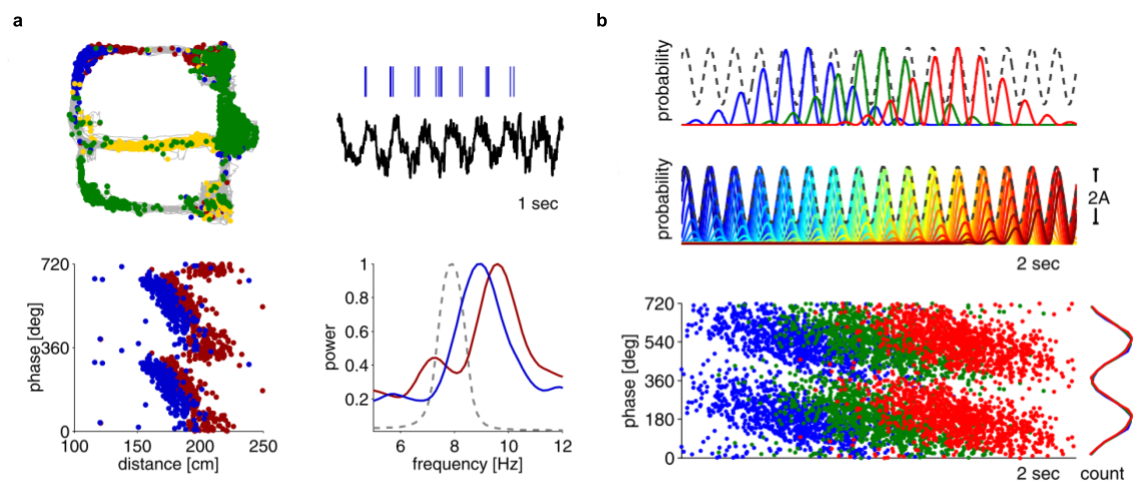
\includegraphics[width=150mm]{figures/F3_phase_precession.png}}
\caption[Theta phase precession]{
(a) A phenomena of the spiking precession of hippocampal neurons relative to the internal LFP theta oscillation. A neuron spiking is chunked by the oscillation and appears earlier in phase as a rat goes through a place field. (b) Sequences of memories and their interference (top), spiking phase relative to the theta oscillation (adapted from \cite{Geisler2010}; permission not required).
}
\label{fig:F3_phase_precession}
\end{figure}



\subsection{Formation of place fields}

Grid, border and head direction cells in the mEC together form one independent representation of space, stable between environments. The reciprocal representation is constructed by hippocampal place cells, that often fully remap between different environments, forming an unique representation of a particular space. These two spatial representations are complementary: one expresses the metric of a space independent of the specific landmarks or action-defined context, another is sensitive to the unique experiences in that space, location of objects or landmarks, building a number of context-dependent orthogonal representations.

The experimental evidence of the increased density of hippocampal place fields near corners and boundaries compared to the center of the environment (\cite{Wiener2737}) leads to a suggestion of a high level of a direct contribution of the border cells to the formation of place fields. Another fact supporting this hypothesis, is that border cells in the mEC are available in the early development - as do place cells when an animal explores an environment on the first day. This leads to an assumption that border cells might have a larger influence on place cells in youth, with the increasing role of grid and other types of mEC cells in adulthood.

Importantly, there is a bidirectional connectivity between hippocampus and entorhinal cortex (see - hippocampal anatomy), the latter receiving feedback from the hippocampus that may be essential for the formation or maintenance of entorhinal spatial maps. This is supported by the experimental evidence that the inactivation of the hippocampal inputs leads to the loss of hexagonal firing pattern of grid cells (\cite{Bonnevie2013}). These facts might be crucial for the explanation of the effects of place cell behavior presented in the results section.

To build experience-dependent representations, place cells need to interact with a variety of entorhinal cell assemblies, carrying distinct types of information. The efficiency and domination of different input types depends on intrinsic properties, like synaptic plasticity, but also on interaction with the environment - animal running speed, behavior, or environmental changes (\cite{Igarashi2014}). It is not yet clear if some of the input types dominate the other, and how place cells recruit synaptic inputs of a certain type to build stable spatial fields. In this work I try to address these questions and to demonstrate that in some particular conditions these inputs of allocentric and idiothetic nature are mixed, and try to further explore the dynamic balance between them.


\subsection{General questions}

The mechanisms that implement spatial navigation in the hippocampal-entorhinal system are not fully described and understood. Among open questions are the mystery behind the formation of the grid patterns, the phenomenon of theta phase precession, the role of gamma oscillations in memory consolidation, how and where the path integration is implemented and many others. Here in this study I focus on the phenomena of place cells in the CA1 region of the hippocampus, especially on the integration of the idiothetic, or precisely boundary-driven information and the visual, landmark driven information into a reliable space representation. The interaction between these allothetic and idiothetic inputs at the level of their postsynaptic influence, especially when they are in conflict, is not yet fully understood. Ultimately, these interactions may reveal, if described in detail, the more general mechanisms of episodic memory formation within the hippocampus which could be extended from navigation to a broad range of behavioral applications, including general action planning and abstract thinking.


\section{The role of visual landmarks and physical boundaries in spatial navigation}
\label{sec:role_of_landmarks}


\subsection{What is a place?}

A place in physical space can be uniquely defined by a set of reference points and landmarks, similar to it’s representative location on an allocentric map. Place is usually considered invariant of time and independent of the way how a subject gets there. This invariance connects the definition of place to the broader definition of semantic memory - invariant stable description of living things, facts or other knowledge (\cite{Buzsaki2013}). Repeated exploration of the environment allows subjects to revisit the same location multiple times, gradually building its representation from recurrent similar episodes - by linking together different (in time) episodes that share the same set of features, landmarks and relations between them.

High-level feature extraction is necessary to build a coherent representation of space, mainly because early sensory systems predominantly encode very simple stimulus modalities with very localized receptive fields. These would not be enough to build similar episodes sharing the same set of features, in case, for example, an animal reached the same location from opposite sides - and  experienced some different visual flow, experienced a set of new sounds, or made a different number of steps walking from the other boundary. Higher brain areas like hippocampus or cortical areas, involved in both memory and navigation, need to operate with higher order features like boundaries, objects of different shape, visual and olfactory landmarks, in order to be able to combine them as a set of similar combinations of sensory features (episodes) to an invariant representation of a particular location. As was shown in the first section, these operations of high-order feature selectivity might mainly reside in the mEC/lEC, being mostly implemented by boundary, object, and landmark vector cells. As anatomically hippocampus receives its major input from the entorhinal cortices, its role in navigation, shown by place cells, might be to orchestrate these incoming navigational information elements to either build and store a new place memory - a unique constellation of features, representing new location, or to update already existing place memory, if this set of features is similar to the already experienced number of stable objects, shapes and cues at a certain distance.

While external sensory information about distinctive and stable environmental features is necessary to build a stable allocentric map, the internal idiothetic information is required to both support this initial formation, as well as to maintain the constructed representation when the external information is partially or completely not available - for example, in total darkness. Our brains are able to maintain the allocentric position and navigate in space without external inputs, for the price of some error accumulation (\cite{Etienne1988}; \cite{Etienne2004a}). This is an indispensable function of the internal navigation system, essential for successful survival and evolution. The implementation of that feature requires an integration of the information coming from the internal idiothetic system into the circuits, encoding spatial maps. This aspect of establishing, recalling and maintaining the spatial map in absence of sensory inputs are discussed below in this chapter.


\subsection{Landmark and boundary vectors as reference frames to establish spatial map}

Overall, to build a spatial map one needs to define a set of related places (in the brain - place fields) having a certain position within a particular spatial reference frame. A reference frame can be defined as an independent coordinate system, having a definite distance and orientation to one or several reference points. Following this classical definition both environmental boundaries and a set of visually defined landmarks can serve as two independent reference frames, if they don’t change their relational stability between reference points within itself. When it is the case, the aforementioned landmark vector cells and boundary vector cells (\cite{Deshmukh2011}; \cite{Hooydal2019}) can be used to represent two reference frames of different modality in the brain.

While exploring the new environment, these inputs from the boundary vector cells and landmark vector cells (as well as other sensory modalities - olfactory, auditory etc.) are integrated to form coherent stable points, or recurrent episodes, which taken altogether, can be used to form a consistent allocentric representation of the surrounding environment. While moving from one place to another, animal revisits the places, formed of the similar set of environmental features, and reactivates the very similar sensory inputs which, with the help of some pattern completion mechanisms, updates and sharpens the CA1 ensemble representation of a particular physical location - place field in the hippocampal memory system. This movement from one place to another builds a trajectory - a set of connected physical places as an animal path, as well as the set of activated and connected places fields as a virtual path in the brain (\cite{Buzsaki2013}).


\subsection{Mechanisms of path integration to support navigation stability}


To maintain the navigational stability when allocentric cues are removed, the internal navigation system, including place cells, continues to track location using self-motion. Path integration is essentially a computation transforming a change in motion into a change in position. Having a current position estimate, one can derive a new allocentric position by tracking angular movements and distance travelled. Whether this system is based on continuous integration of angular or linear velocities, or on addition of a distance travelled vector to the current estimate - it is based on cues derived from the inputs from the self-motion systems (\cite{Etienne2004a}). These cues include vestibular, proprioceptive cues or motor efference copy (step counting). Additionally, a change in airflow (e.g. sensed by whiskers) or vibration from textures while moving can support speed calculation and resulting translation detection (\cite{Savelli2019}).

How can the path integration system be implemented in the brain circuits? While both distance and angular movement signals coming from grid and head direction cells tend to drift in open spaces without correction by particular cues or landmarks (\cite{Barry2007}), they are still the great candidates to support the path integration system. Boundary cells, or the tactile sensory inputs in the environmental corners, can episodically reset the grid and head direction inputs bringing the path integration system up to date with the environment position and orientation (\cite{Barry2007}; \cite{Cheung2012}). This leads to an assumption that path integration is mainly implemented in the cerebral cortex in a form of an attractor-network (\cite{Knierim2012}; \cite{McNaughton2006}), supported by the fact that the hippocampal upstream regions have all necessary components.

Another reported alternative is that the path integration computations are performed in lower regions, subcortically, reflecting the organization of the head direction system (\cite{Savelli2019}). As thalamic or other subcortical regions already receive vestibular and motor signals, they are able to compute and integrate angular and translational velocity signals, implementing basic path integration. The anatomical structure of the head direction system, for instance, with head direction cells found in anterior dorsal thalamic nucleus (\cite{Taube1995}) is another evidence to support this alternative.


\subsection{Impact on place cells}

Navigation at the level of hippocampal formation with its place cells are the main focus of this study. There is evidence showing that place cells follow visual cues (\cite{Muller1987}; \cite{Deshmukh2013}; \cite{Aronov2014}), suggesting that they receive incoming allocentric information. There is also a large evidence showing that place cells are able to maintain their place preference in case the sensory inputs are removed (\cite{Gothard2001}; \cite{Quirk1990}). In conflicting situations, as was shown in virtual reality (VR) studies (\cite{Gothard2001}; \cite{Haas2019}), cells are able to switch from one to another reference frame in their selective firing, suggesting integration of allothetic and idiothetic inputs. As described in the previous sections of this chapter, initial sensory processing and feature extraction, as well as path integration happens mainly outside the hippocampus. Taken together - how exactly these different pathways are integrated within the hippocampal neural circuits? This question is still not well understood. Below I review a few model studies exploring potential mechanisms of this integration (see modelling section).


\section{Research on interaction of allothetic and idiothetic inputs}
\label{sec:interaction_allo_idio}

One of the first seminal research studies of the effect of the allothetic environmental changes on place cells was done in 1987. Muller and Kubie (\cite{Muller1987}) showed that the rotation of a visual cue card, but not its width or shape, produces rotation of the place fields in a cylindrical arena. Removing the card led to a randomized angular representation of the arena. These recordings demonstrated direct dependence of the place field orientation on the visual information, implicating that cells in the hippocampus are modulated by allothetic visual inputs.

Getting more detailed, several years later, it was shown that objects located near the center of the arena could not control the orientation of the place fields in the environment, but do that with a help of a cue card on the wall (\cite{Cressant1997}). Same objects, placed near the walls enable control over the fields orientation, indicating that involvement of the head direction system, that potentially resets angular orientation relative to the unique objects, located close to the environmental borders.

The question of interaction of allocentric and idiothetic representations got more specificity in later studies by Bures and Zahalka (\cite{Bures1998}), where they experimentally trained animals to avoid foot shocks using either room landmarks or using idiothetically defined area on the floor. The ability of rats to avoid shock locations defined in both reference frames showed credible independence of the allocentric and idiothetic mechanisms, encoding two reference frames. However, a question of how these two systems are intermixed remained unclear.

Gothard and McNaughton proposed that place cells, mainly driven by internal “path integrator” - accumulated internally-driven translational information about a movement in space together with head direction cells - form a preconfigured network of a two-dimensional space. This network is updated by the visually-specific landmark information using associative learning (\cite{Mcnaughton1996}). They performed a series of experiments with rats on the linear track where two separate reference frames were used by a rat to track self position. By gradually moving these reference frames (a reward site and a starting box), they found both cells fired at fixed distances from the origin and cells fired at proximity to the destination. The same neuron was able to shift its spatial preference from being aligned to the origin to an alignment to the destination. They postulate that when mismatches between the visual and the idiothetic information occur, path integration and sensory cues competitively interact to affect place field preference (\cite{Gothard1996}). Their further recordings in light and dark conditions, showing that the box-referenced cells tend to keep their firing preference longer even without light, supported that idea. Ultimately, based on their moving-box-reward experimental data they suggest that interaction between internal dynamics and path integration and external sensory cues happens before both CA1 and CA3 areas, possibly in the entorhinal cortex or subiculum.

However the question of exact mechanism of position computation based on actual or path integrated information remained unclear. A new set of tools including virtual reality was introduced to continue the research of dynamics and circuitry implementing allocentric- and idiothetic- based navigation.


\begin{figure}
\captionsetup{format=plain}
\makebox[\textwidth]{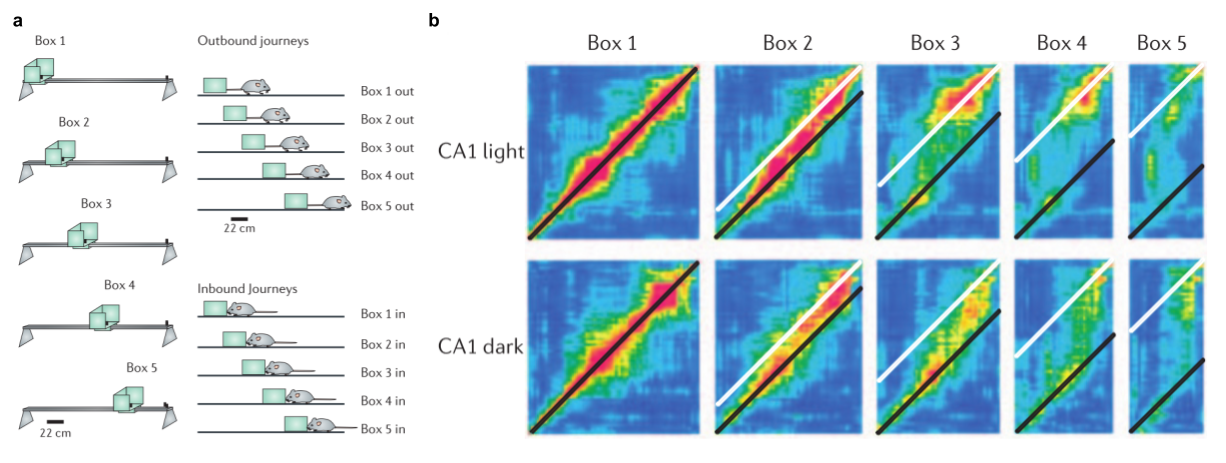
\includegraphics[width=150mm]{figures/F4_moving_box.png}}
\caption[Moving shelter as a reference frame]{
(a) A schematic of the experiment with a moving box. A starting box together with a reward location at the end of the track act as two independent reference frames. By gradually moving the box one can investigate the change of the spatial encoding relative to either of the frames. (b) The resulting place cell firing in light and dark establish gradual shift in encoding position (adapted with permission from \cite{McNaughton2006})
}
\label{fig:F4_moving_box}
\end{figure}


\section{Optimal combination of environmental cues and path integration during navigation}
\label{sec:optimal_comb_for_spat_nav}

How algorithmically do the allocentric and idiothetic inputs merge at the level of the hippocampal place cells? When the brain needs to integrate information of different sensory modalities it often uses “optimal” combination - a weighted sum of the inputs with weights proportional to their reliability. This has been established in many behavioral and theoretical studies for humans (\cite{Ernst2002}; \cite{Alais2004}; \cite{Knill2003}; \cite{Hillis2004}) for combinations of different sensory modalities (visual / auditory, visual / haptic, stereo / texture, environmental geometry / path integration etc.). The optimal coding theory is also applicable for spatial navigation. In a series of behavioral studies position estimation based on Bayesian decoding was established and predicted. In particular, optimal cue integration is demonstrated in ants (\cite{Wystrach2015}), rats  (\cite{Shettleworth2005}) or humans (\cite{Zhao2015}; \cite{Chen2017}; \cite{Sjolund2018}). However, while real-world navigation normally implies redundant integration of external, allocentric, cues and internal, idiothetic or path-integration based position estimations, is that combination always optimal?


\begin{figure}
\captionsetup{format=plain}
\makebox[\textwidth]{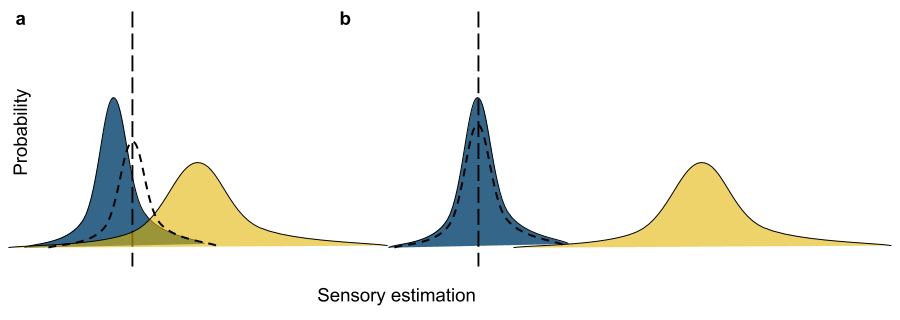
\includegraphics[width=150mm]{figures/F5_larger_smaller_conflicts.png}}
\caption[Sensory conflicts of different size]{
Sensory integration at larger and smaller conflicts. (a) In a situation of a small conflict between estimations it is beneficial to use optimal coding - a weighted combination of the estimation with weights proportional to their reliability (variance). Also named Bayesian decoding, or maximum likelihood estimation (MLE). (b) In a situation of a large conflict between estimations a strategy of abandonment of a less reliable information source will have higher chances to end with a better precision.
}
\label{fig:F5_larger_smaller_conflicts}
\end{figure}


Intuitively, when the conflict between two given estimations is small, weighted integration and resulting averaging makes sense. Especially if performed in an optimal, Bayesian way, it allows for a maximization of the precision of the resulting estimate, attributing a conflict to a sensory noise (Figure 5a). On the other hand, situations of a large conflict might be caused by misidentification of an object identity, incorrect memory retrieval or in general - failure in estimation based on a particular sensory source. In that case Bayesian integration might lead to large errors relative to both information sources, while full abandonment of one, ideally less reliable, source of estimate might be a logical choice (Figure 5b). This abandonment of one source, or cue, in favor of the other has been demonstrated in animal and human navigation studies. For instance, when humans were presented with a large > 115 degrees conflict between landmark and path integration cues they prefered path integration (\cite{ZHAO201596}). Rats in large spatial conflicts also prefer to rely on path integration in favor of a single landmark (\cite{Shettleworth2005}).

While the ability of a brain to implement optimal coding is well known, however it has not been thoroughly explored at the physiological level. Different potential schemes, including gain field theory, convolutional encoding, doubly distributional population coding were introduced (see review in \cite{Pouget2003}), however it is still not clear which scheme is used by the neurons or whether neurons actually encode continuous distributions at the population level. In this work, we address this question and make an attempt to show on the cellular level how these mechanisms of estimation integration at small conflicts and estimation abandonment at large conflicts could be implemented by a population of hippocampal neurons. We hypothesize that attractor dynamics in the hippocampal circuits might implement nearly-optimal coding for spatial and potentially non-spatial estimations, predicted earlier in other sensory systems (\cite{Jeffery2016}) and how the abandonment of less reliable estimation could be implemented at the level of a single neuron.


\section{Modelling multisensory integration at the level of place cells}
\label{sec:modelling}

“…Each place cell receives two different inputs, one conveying information about a large number of environmental stimuli or events, and the other from a navigational system which calculates where an animal is in an environment independently of the stimuli impinging on it at that moment. The input from the navigational system gates the environmental input, allowing only those stimuli occurring when the animal is in a particular place to excite a particular cell…” - an original sentence by O’Keefe led to a general proposal that the place cells might integrate idiothetic information coming from the different cell groups from the entorhinal cortex with some other sensory information.

Initially, a discovery of grid cells led to a model proposed by Solstad and Einevoll, which assumed formation of place cells via linear summation of weighted inputs from the grid cells (\cite{Solstad2006}). It was suggested that irregularly spaced place fields can appear as a result of summing inputs from entorhinal cells with different spacing and orientation, and relatively similar grid phases. However, this model was free from complex network interactions and required having place cells integrating grid cell inputs with overlapping vertices. This issue was fixed later by demonstrating that adding fast hebbian plasticity may result in the careful selection of appropriate inputs, without the need for specific network wiring (\cite{Savelli2010}).

The discovery of border cells and boundary vector cells led to another approach, assuming that environmental boundaries can serve as determinants of the hippocampal place fields. The boundary vector cell model (\cite{Barry2006}) describes place fields emerging from a combination of cells active at a certain direction and orientation relative to the environmental boundaries.

However, both of these approaches were focused on feed-forward type of information transfer, uni-directional communication between cortex and hippocampus. Recently, a novel approach connecting feed-forward information flow from the entorhinal layers to the hippocampus with feedback flow to the entorhinal areas, was proposed (\cite{Li2020}). It is a model that assumes continuous interaction between grid and place cells, with plasticity mechanisms enabling balance in control over place definition between vision and self-motion, allocentric and idiothetic inputs. In this model, self-motion is represented by multiple layers of grid cells that integrate angular and translational movement velocities (see grid cells). Visual input is modelled using a retina-like grid with Gabor filters, applied to the incoming stream of camera images. It is also assumed that it gets input from the head direction system such that the resulting visual information in particular location is independent from head orientation, similar to the non-grid cell in the lEC (see object-vector cells). Competitive organization of the network outputs establishes two different populations of place-selective cells - purely self-motion (or boundary) driven (motion place cells - MPCs), and purely visually driven (visual place cells - VPCs). These cells are assumed to be present in the CA3 regions of the hippocampus and together provide informative inputs to CA1 place cells. Having hebbian plasticity mechanisms and feedback connections back to the self-motion grid cells (MPCs), these latter CA1 cell are classified into 3 major groups - visually driven, self-motion or boundary driven and multisensory cells, that combine both of the allothetic and idiothetic inputs. These simulation results are very similar to the previously reported results (\cite{Haas2019}), as well as they highly correlate to the new electrophysiological data from the current study. Here I found very similar groups of neurons, having similar spatial firing properties (see Results). However, the disadvantage of the model is that it does not account for border-defined inputs which, as we also find in the neural data, might play an important role in correcting self-motion vectors and modulating the dynamics of the network as a whole.

Ultimately, considering models of the underlying neural dynamics, the current work is attempting to provide additional evidence for the modern loop-based approach to describe hippocampal-entorhinal networks implementing principles of spatial navigation. Based on the collected data, we hypothesize that hippocampal neurons implement a weighted combination of position estimation based on allocentric and idiothetic inputs in a nearly-optimal fashion. We show that the resulting position estimation influences self-motion based place representation, possibly via backprojections from the hippocampus to the entorhinal cortex. Overall this makes a step towards bringing evidence based on the neurophysiological data for the proposed model in situations, when place definitions are conflicting.


\section{Aim of the thesis}
\label{sec:aim_of_thesis}

For many years hippocampus has been identified as a brain structure, critical for spatial learning and navigation. The spatial domain extends beyond the traditional navigation in physical spaces - to many abstract spaces humans need to operate daily, not only to be partially efficient, but also to be successful in survival. Hippocampus, having specially tuned neurons - place fields - that rely on external sensory inputs and self-motion cues, mainly coming from the cortical areas, is able to implement high-level context-dependent representation of the environment. However it is still not known how exactly these different information flows interact to build a consistent and stable map of connected place fields.

Existing studies suggest that both proprioceptive and idiothetic types of information are continuously integrated to update the self-position (e.g. implementing “path integration”) while other stable sensory cues provide references to periodically update the allocentric position of self and correct it for the collected integration-related errors. It was shown that both allocentric and idiothetic types of information influence positional cell firing, however in most of the studies these inputs were firmly coupled. The use of virtual reality setups (\cite{Thurley2016}) made it possible to separate the influence of vision and proprioception for the price of not keeping natural conditions - the animal is usually head- or body-fixed (\cite{Holscher2005}; \cite{RavassardA.2013}; \cite{Jayakumar2018}), which introduces vestibular motor- and visual- conflicts, providing a bias for space encoding. Here we use the novel CAVE Virtual Reality system for freely-moving rodents (\cite{DelGrosso2018}) that allows to investigate the effect of visual- and positional- (vestibular) manipulation on the hippocampal space code while keeping natural behaving conditions.

Particularly, the current research is aimed at studying the impact of visual and vestibular (passive translation) manipulations on the hippocampal code using this novel freely-moving ratCAVE system. With the ability to manipulate the projected virtual environment and to unidirectionally move the physical arena depending on animal’s position, the following questions are addressed:

\begin{itemize}
  \item how would the stable visually-defined spatial reference frame impact the hippocampal place code when put in conflict with the moving space reference frame, defined by the physical boundaries
  \item would the passive physical move in space, locked to the physical boundaries and supported with vestibular inputs, differently impact the place code in contrast to the opposite situation when the move of the reference frame is just visual and not supported by the vestibular inputs - addressing the question of the role of vestibular information in coding the preference to one or another reference frame
	\item whether an instant mismatch between the visual and proprioceptive inputs (gain) would distort the hippocampal place map and at which threshold
	\item what types of the hippocampal place cells could be separated by their sensory and / or feedback inputs (visual, self-motion or boundary-driven or their combinations) and how strong is the path integration component
	\item whether a single instant conflict between information coming from the internal path integration system and the visual information can influence the current place code or lead to any remapping
\end{itemize}

In summary, we focus on the dynamic representation of space when the visual-cue-defined and physical-boundary-defined reference frames are in conflict. We confirm the dominance of one reference frame on the other on the level of place fields, when the information about one reference frame is absent (\cite{Gothard2001}). We show that the hippocampal cells form distinct categories by their input preference - surprisingly, not only that they are being driven either by visual / allocentric information or by the distance to the physical boundaries and path integration, but also by a specific combination of both. I found a large category of units integrating inputs from both allocentric and idiothetic pathways that are able to represent an average location between two reference frames, when they are in conflict. The use of virtual reality allowed me to demonstrate that these units become only path integrator driven when they lose their visual inputs. Based on the recorded information about these single cell theta phase-modulation, I propose a model how these units can integrate allocentric and idiothetic inputs to form this independent category of place representation.

Ultimately, the aim of the current work is to try to provide more support in linking the view over the hippocampus from the other side - to consider it not only as a spatial machine, but as a common generator of sequences of episodic memories (\cite{Buzsaki2013}), having place cells as examples of a particular recurrent episode - an integrated internal and external feature-processed sensory information at a particular moment of time, shaped by brain theta rhythms.
